%Requires the memoir class 
\documentclass[oneside,11pt]{memoir}

%\usepackage{mathptmx}  % Times New Roman, but if you have Garamond then use it;
                        % you are writing a book, not a newspaper column

\DoubleSpacing        % memoir's double spacing
\usepackage{rice}     % rice thesis package 


\usepackage{graphicx}
\usepackage{rotating}
\usepackage{amssymb}

\usepackage{txfonts}  % I used this one to summon the symbol for \lambdabar
\usepackage{lmodern}

\usepackage[numbers,compress]{natbib}

\usepackage{hyperref}
\usepackage{memhfixc}

%%%% Definition of command shortcuts %%%%
\newcommand{\twos}[1]{\ensuremath{\hspace{-1pt}2\hspace{0.5pt}\hspace{0pt}S_{#1}\hspace{-1pt}}}
\newcommand{\twop}[1]{\ensuremath{\hspace{-1pt}2\hspace{0.5pt}\hspace{0pt}P_{#1}\hspace{-1pt}}}
\newcommand{\trep}[1]{\ensuremath{\hspace{-1pt}3\hspace{0.5pt}\hspace{0pt}P_{#1}\hspace{-1pt}}}

\newcommand{\cm}{\ensuremath{,\hspace{1pt}}}
\newcommand{\f}[1]{\ensuremath{F\hspace{-5pt}=\hspace{-4pt}#1}}
\newcommand{\mf}[1]{\ensuremath{m_{F}\hspace{-4pt}=\hspace{-4pt}#1}}
\newcommand{\mj}[1]{\ensuremath{m_{J}\hspace{-5pt}=\hspace{-4pt}#1}}
\newcommand{\mcm}{\ensuremath{\hspace{-4pt}}}

\newcommand{\red}{\ensuremath{ \twos{1/2}\hspace{-0.0pt}\rightarrow\hspace{-0.0pt}\twop{3/2} }\ }
\newcommand{\uv}{\ensuremath{ \twos{1/2}\hspace{-0.0pt}\rightarrow\hspace{-0.0pt}\trep{3/2} }\ }

\newcommand{\TD}{\ensuremath{ T_{D} }}
\newcommand{\TR}{\ensuremath{ T_{R} }}
\newcommand{\TF}{\ensuremath{ T_{F} }}

\newcommand{\one}{\ensuremath{|1\rangle }\ }
\newcommand{\two}{\ensuremath{|2\rangle }\ }

\newcommand{\isat}{ \ensuremath{ I_{\mathrm{sat}} } } 
\newcommand{\isatred}{ \ensuremath{ I_{sat\text{(red)}} } } 
\newcommand{\isatuv}{ \ensuremath{ I_{sat\text{(uv)}} } } 

\newcommand{\li} {\ensuremath{^{6}}Li\ }

\newcommand{\kb} { \ensuremath{k_{\mathrm{B}}}}


\DoubleSpacing

\begin{document}

\maxtocdepth{subsection}   % put everything into the ToC
\pagestyle{plain}          % pagestyle for the prelims

\frontmatter
\thetitlepage

%%%%%%%%%%%%%%%%%%%%%%%%%%%%%%%%%%%%%%%%%%%%%%%%%%%%%%%%%%%%%%%%%%%

% put your abstract here

\riceabstract
\pagestyle{empty}  % Rice requires no page numbering in the abstract

Abstract goes here. 

\pagestyle{plain} % Restore page numbering.

% put your acknowledgements here 
 
\riceacknowledgements

Acknowledgements go here. 

%% \setdedication{ text } % if you want a dedication
%\ricededication

%\tableofcontents
\tableofcontents*  % The starred version does not add "Table of Contents" to the Table of Contents
                   % I prefer it this way


% I don't find these two particularly useful
%% \listoffigures  % if you want to include a list of figures  
%% \listoftables   % if you want to include a list of tables


%% if you have more prelim sections, then
%%%% \clearpage
%%%% \pagestyle{plain}
%%%% \prelimtitle   text % for sections after the ToC, etc, before main text


\mainmatter
\pagestyle{rice}


%% Change the spacing between paragraphs, I prefered this for readability 
\let\oldparskip\parskip
\setlength{\parskip}{0.8em}


\chapter{Many body physics with ultracold atoms } 

\section{ Motivation:  Strongly correlated materials }

Our experiences in the physical world can, for the most part, be explained by
considering the description of the collections of positively charged nuclei and
negatively charged electrons that make up ordinary matter.    From high to low
energy this includes neutral plasmas,  the formation of atoms and molecules in
gaseous phase, the condensation of these atoms and molecules into liquid or
glassy phases and their susequent crystallization to form solids.   At lower
energies more exotic phenomena take place, starting with magnetism and going
further to superfluidity, superconductivity and the novel examples of modern
condensed matter physics such as the fractional quantum Hall effect, heavy
electrons, high-temperature superconductors and topological insulators.

In principle,  the correct description of all the above phenomena is contained
in the Schr\"{o}dinger equation for the interacting system of electerons and
nuclei,  where the interaction is given by the Coulomb potential. In practice,
we know that even though stating the equation is easy, there is not sufficient
computing power available in the world to solve it for systems of more than
just a few particles.  In the introduction to his book~\cite{wen2004quantum},
Xiao-Gang Wen points out that back in the 80s a computer with 32 MB of RAM
could solve a sytem of 11 interacting electrons.  In the 2000s, while computing
power has increased more than 100 times, this allows for the addition of only
two more electrons to the system.  

Despite the above,  the use of the Schr\"{o}dinger equation and perturbation
theory for the description of  systems of electrons and nuclei has been very
succesful over the past century.  The most prominent example of this success is
our understanding of semiconductors, which are at the root of the electronic
devices that permeate all aspects of our lives.  The remarkable success of this
approach can be traced back to the principle of adiabatic
coninuity~\cite{altland2010condensed}, which states that the quasiparticle
low-energy excitations of an interacting system can be closely related to the
particles that form the interacting system.  

The practical consequence of adiabatic continuity is that interactions
seemingly do not play an important role in the low-energy description of the
system.  For this reason, the free electron model of Drude and
Sommerfeld~\cite{ashcroft1976solid} was relatively succesful in explaining
electrical and thermal conductivity in metals and the Hall effect.   Later on,
in 1957, Landau formulated the thery of the
Fermi-Liquid~\cite{landau1965collected} and gave a solid basis to the notion of
adiabatically connected quasiparticles.  To this day, the Fermi-Liquid theory
is the starting point for the study of Fermi systems such as conventional
metals, $^{3}$He and ultracold atomic Fermi gases.

Just as Fermi-Liquid theory is celebrated for its success it is also known for
the phenomena that it fails to explain.   Starting in the mid 70s and going
through the 80s, the discoveries of heavy electron
superconductivity~\cite{PhysRevLett.35.1779,PhysRevLett.43.1892},  the
fractional quantum hall effect~\cite{PhysRevLett.48.1559,PhysRevLett.50.1395},
and high-temperature superconductors~\cite{Zeitschrift.64.189} sparked a
revolution in condensed matter physics~\cite{coleman2004revolution}.   These
materials in which the electron behavior cannot be described effectively in
terms of non-interacting electron-like quasiparticles came to be known as
\textit{strongly correlated materials}.   Strongly correlated  materials and
the concept of emergence, introduced by P.W.~Anderson in his famous essay
``More is Different''~\cite{Anderson1972}, are at the center of modern
condensed matter physics. 

The behavior of strongly correlated materials is emergent because the
low-energy excitations of the system bear no resemblance to its constituent
particles.  This concept should not be so surprising, after all we are familiar
with this definition of emergence whenever a system undergoes a phase
transition.  For example when a liquid transitions to a crystalline solid,
translational symmetry is broken  and the low-energy excitations of the system
are the quasiparticles known as phonons, which bear no resemblance to the
constituent ions and electrons that form the solid.   

Strongly correlated materials are are examples of emergent phenomena in which
the origin and properties of the low-energy excitations are not as
straightforward as those of phonons in a crystalline solid.  The fractional
quantum Hall state, in which the quasiparticles carry a rational fraction of
the charge of an electron serves to illustrate this point.  The strong
interactions between the electrons in the quantum Hall system (electrons
confined in a plane under a very high magnetic field) make the problem
intractable from the perturbative point of view and thus the connection between
the microscopic degrees of freedom and the collective low-energy excitations is
very difficult to establish; certainly not as easy as the connection between
the small motion of ions about their equillibrium positions in a crystal and
their collective phonon modes. It was Laughlin's insight that led him to
postulate the correct wavefunction  for the quantum Hall
state~\cite{PhysRevLett.50.1395}, but the microscopic origin of the state is
still under debate.   

The challenge posed by strongly correlated materials has led to great
discoveries in condensed matter physiccs, such as the concepts of topological
order~\cite{wen1990topological} and quantum
criticality~\cite{PhysRevB.14.1165,sachdev2011quantum}, but also many questions
remain unanswered.  Furthermore, the problem of strongly correlated materials
is only scratching the surface of what is possible and what remains to be
discovered.  New materials are being synthesized constantly, and among the
myriad of possible materials and compunds that can be explored by materials
scientists, one can only expect that there will be new states of matter to be
found and ones with technological implications that will revolutionize life on
earth.  


\section{Quantum simulations with ultracold atoms}

We have seen that even though the Schr\"{o}dinger equation in principle
contains a full description of a solid,  the solution is practically impossible
to compute using a classical computer due to large memory required to represent
many-body quantum state.   
%Beyond this issue of scalability there is also the
%issue of interpretation of the results:  suppose that we were able to access
%the exact quantum state of the system and its time dependence,  what would we
%even do with such information?   It would be practically impossible to come up
%with experiments that could test the full validity of the state, thus making
%such knowledge superfluous since, after all, physics is an empirical endeavor.
The approach in condensed matter theory, rather than directly aim to solve the
Schr\"{o}dinger equation, is to introduce simplified effective models, which
should capture the essential features of the system under study.  The solution
of the effective model leads to an understanding of the low-energy excitations
of the system and gives clues to their microscopic origin.   

The Hubbard model is a model that contains only the essential ingredients
to describe the  behavior of strongly interacting electrons in a crystalline
solid.    The model describes electrons that can hop between sites in a
lattice, and which acquire an interaction energy when two electrons are on the
same site, see Figure~\ref{fig:chap01hubbard}.  
\begin{figure} \centering
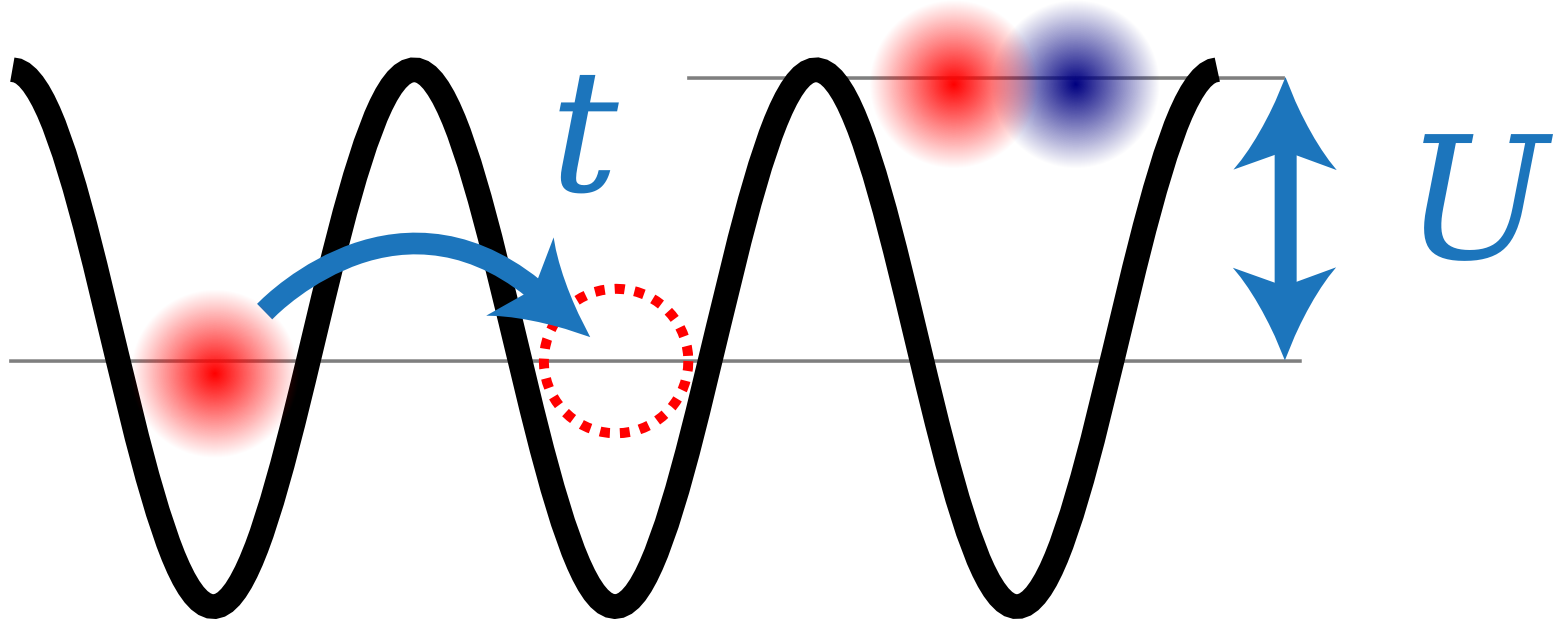
\includegraphics[width=0.4\textwidth]{../figures/hubbard/little-hubbard.png}
\caption[Hubbard model]{\small Illustration of the Hubbard model }
\label{fig:chap01hubbard}
\end{figure}
In the next chapter I will explian why this is a plausible model to
describe some strongly correlated materials;  for know I will point out that
even though this model is the simplest possible model for strong correlations
its solution in more than one dimension has evaded theorists for more than four
decades.

It is at this point that ultracold atoms enter the picture.   It turns out that
a system of ultracold atoms in an optical lattice is a faithful realization of
the Hubbard model~\cite{PhysRevLett.81.3108}, and so the properties exhibited
by the atoms are in fact the solutions of the model.   The idea of studying the
solutions of a quantum mechanical model using an analogous quantum mechanical
system was first proposed by Richard Feynman in
1982~\cite{feynman1982simulating} and has been made possible in the last decade
due to the advances in production and control of ultracold atomic gases.   Besides the ability to cool atoms to temperatures that are only a 5\% of the Fermi temperatures,   the success of the field is due to the ability to create periodic potentials for the atoms by interefering laser beams and also due to the fact that the interactions betwen the atoms are contact interactions.

Interactions are contact.   

Lattice depth can tune U/t  (bosons) 
 
Feshbach resonances, can tune interacions (cesium, fermions)  

Challenges, temperature:  both cooling and thermometry

Approaches:  compensation,  spin sensitive (this thesis)  



%The Fermi-Hubbard model was formally presented to the world by Hubbard in his
%1950 paper titled ``whatever''.  Perhaps he could suspect at the time that he
%was then fathering a model that to this day remains at the center of condensed
%matter physics.   

In this section I present the model in its original context, as a
simplification of the description of valence electrons in crystalline solids.
I include some historical background to motivate the reader.  

Models for electrons existed which explained conduction phenomena in a
succesful manner.  Also, models existed which dealt with magnetic phenomena.
This section touches on the necessity to formulate a model that could
incorporate both transport and magnetic properties of a material.   This need
arises due to the existence of materials that are at neither end of the
spectrum.  That is, metals or insulators for which magnetic effects played an
imporant role.   The simple example being MnO, on which antiferromagnetism was
first observed,  and the big challenge being high-temperature
superconductors. 

\section{ Motivation:  Quantum magnetism with ultracold atoms }

An overview of the literature for observation of quantum magnetism in ultracold
atoms

\chapter{The Fermi-Hubbard model}

\section{ The Hubbard model in ultacold atomic gases }

This section starts by considering the description of cold atoms in an optical
lattice potential.  It then considers interactions on the description of the
system.  The main point of this section is to make the reader aware of  what
are the approximations that are made whene one says the system of interacting
atoms in an optical lattice is described by the single band Hubbard model.   

\subsection{ Motion of atoms in an optical lattice potential }
\subsection{ Interactions between the atoms }  

\section{Simplified treatements}

This section explains our understanding of the Fermi-Hubbard model.  It starts
by building some insight by using the results of exactly solvable models.   The
results of exct diagonalization in systems of 2-sites and 4-sites are shown.
This are going to motivate the antiferromagnetic character of the ground state,
while showing that there is always a bit of an admixture of double occupancy in
the exact ground state.  

The 4-site solution can be used to help understand why the Fermi-Hubbard is relevant to high-Tc superconductors.   In this case one can make connections to the $d$-wave character of ground states upon doping the system.   

The exact diagonalization solutions are at zero temperature, so they give most
insight to the exact ground states of the system. 

\subsection{ Exact diagonalization } 
\subsubsection { 2 site exact diagonalization } 
\subsubsection { 4 site plaquete an relevance to high-Tc superconductors}

\subsection{ Limiting cases} 

This section deals with the limiting cases of the Fermi-Hubbard parameters.
The solutions that are obtained give insights to the workings of the model.
The high temperature series expansion is introduced, which is very relevant for
calculating thermodynamic quantitites in the temperature regime of a few times
$T_{\mathrm{Neel}}$.  

\subsubsection { U=0 limit, t=0 limit } 
\subsubsection { High temperature series expansion, band and Mott insulating states  }
\subsubsection { small t, the t-J model and antiferromagnetic ground state}

\subsection{Modern approaches}  

This small section aims to explain the most recente advances in our
understanding the Fermi-Hubbard model.  This includes QMC, DMFT, etc.  The aim
of this section is not to provide an introduction to these techniques but
mainly to point out the main results and serve as a bibliographic reference.  


\chapter{Enlarging and cooling towards the Neel state in a compensated optical
lattice potential}

\section{Compensated optical lattice} 
\section{Thermodynamic quantitites in the local density approximation} 


\chapter{Experimental diagnostic tools} 

This chapter aims to describe in detail the different observables that are
accesible to the experimetnalist.  

\section{Absorption imaging} 

\section{Polarization phase-contrast imaging} 

\section{Thermometry of a Fermi gas trapped in a harmonic potential} 

\section{Double occupancy measurement in an optical lattice }

\section{Bragg Scattering of light}
 
\subsection{ Non-spin sensitive: crystal structure factor}
\subsection{ Spin sensitive:  spin-structure factor} 

\chapter{Experimental setup and procedures} 

\section{Production of a deeply degenerate $^{6}$Li spin mixture in a dimple potential } 

\section{Compensated optical lattice potential} 

\chapter{Studies in a three dimensional optical lattice} 

\section{Determination of the crystal structure factor using Bragg scattering}
\section{Insulating states in an uncompensated lattice} 
\section{Evaporative cooling in a compensated optical lattice} 
\section{Detection of antiferromagnetic correlations in a compensated optical lattice}

\chapter{Conclusion} 

%\section{Compensated optical lattice }
%
%\chapter{Realizing the Fermi-Hubbard model with ultracold atoms}
%
%\section{Optical lattice potential}  
%
%\section{On-site interactions} 
%
%\section{Compensated lattice: Enlarging the Neel state} 
%
%
%\chapter{Measurement and diagnostic techniques}
%
%\section{Polarization phase-contrast imaging}
%
%
%\section{Thermometry} 
% 
%\section{Bragg scattering of light}
%
% 
%\chapter{Experimental apparatus}
%
%\section{Magneto-Optical Traps}
%\section{Magic Wavelength Optical Dipole Trap}
%\section{Compensated Optical Lattice}
%\section{Bragg scattering setup} 
%
%
%\chapter{Detection of antiferromagnetic correlations}




%% finally, start of your main text

% if appendices, then
%\appendix
%\chapter{Appendix}


% if Biographical sketch then
%\begin{biosketch}
%I was kissed by a donkey when I was 5..... and text and more text and even more text, lots of text, here and there, more and more text, with more and more descriptions of text, blah etc blah et
%\end{biosketch}

\bibliographystyle{osa}
% Other options for the bibliographystyle are listed below
%\bibliographystyle{unsrt}
%\bibliographystyle{unsrtnat}
%\bibliographystyle{apsrev}
\bibliography{pmd}

\end{document}

